\scanpage{6}

$\unsure{\mathcal{X}|\mathscr{X}}$ qui est aussi la somme amalgamée de\deleted{\unsure{s}} $\overline W$ et de\deleted{s} $\coprod_{i\in I}\overline U_i$ (\unsure{sur}
\diagram{\begin{tikzcd}[ampersand replacement=\&,row sep=small,column sep=large]
\coprod_i B_i \arrow[r,hook] \arrow[dr] \& \overline W\\
\& \coprod_i\overline U_i
\end{tikzcd}}
) :

\noindent\begin{minipage}[c]{.41\linewidth}
\figure{\resizebox{\linewidth}{!}{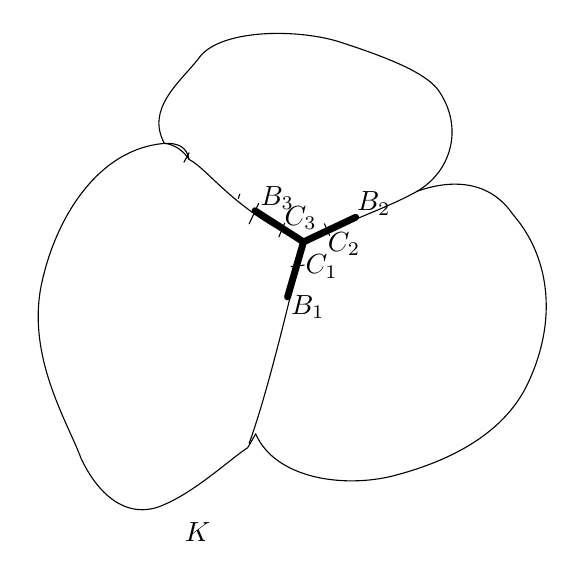
\begin{tikzpicture}[x=.92cm,y=.92cm,line cap=round,line join=round]
\draw (-1.92,1.36) .. controls (-2.18,1.84) and (-1.71,2.20) .. (-1.45,2.53)
 .. controls (-1.18,2.93) and (-.14,2.95) .. (.47,2.77)
 .. controls (1.09,2.57) and (1.65,2.36) .. (1.85,2.11)
 .. controls (2.22,1.60) and (2.05,.98) .. (1.57,.70);
\draw (-1.92,1.36) .. controls (-2.88,1.28) and (-3.46,.25) .. (-3.63,-.65)
 .. controls (-3.80,-1.63) and (-3.25,-2.50) .. (-3.07,-2.99)
 .. controls (-2.81,-3.54) and (-2.39,-3.85) .. (-1.91,-3.62)
 .. controls (-1.47,-3.43) and (-.99,-2.98) .. (-.77,-2.84) -- (-.66,-2.65);
\draw (-.66,-2.65) .. controls (-.38,-3.29) and (.62,-3.41) .. (1.31,-3.21)
 .. controls (2.26,-2.95) and (2.87,-2.50) .. (3.13,-1.88)
 .. controls (3.51,-1.02) and (3.38,-.18) .. (2.89,.38)
 .. controls (2.57,.85) and (2.05,.87) .. (1.57,.70);
\draw (-1.92,1.36) .. controls (-1.78,1.35) and (-1.65,1.25) .. (-1.58,1.14)
 .. controls (-1.30,.99) and (-.96,.44) .. (0,0);
% Narrow return loop at the upper-left outer junction: both edges are visible.
\draw (-1.92,1.36) .. controls (-1.75,1.37) and (-1.61,1.32) .. (-1.58,1.14);
\draw (0,0) .. controls (.67,.31) and (1.20,.49) .. (1.57,.70);
% The descending divider stops short-left of the lower outer cusp.
\draw (0,0) .. controls (-.23,-.96) and (-.51,-2.12) .. (-.75,-2.78);
\draw[line width=2.5pt] (-.67,.43) -- (0,0) -- (.72,.34);
\draw[line width=2.5pt] (0,0) -- (-.22,-.76);
\draw (-1.65,1.10)--(-1.58,1.23) (-.90,.60)--(-.88,.66) (-.75,.25)--(-.62,.53)
 (-.34,.07)--(-.26,.26) (.36,.09)--(.29,.25) (-.17,-.34)--(.01,-.32);
\node at (-.36,.60) {$B_3$}; \node at (-.04,.33) {$C_3$};
\node at (.97,.53) {$B_2$}; \node at (.56,-.03) {$C_2$};
\node at (.25,-.34) {$C_1$}; \node at (.06,-.90) {$B_1$};
\node at (-1.46,-4.00) {$K$};
\end{tikzpicture}}}
\end{minipage}\hfill
\begin{minipage}[c]{.56\linewidth}
\deleted{L'application \unsure{naturelle}}

\[
\deleted{\unsure{\text{de}}\quad\mathcal{X}\longrightarrow X}
\]

\[
\resizebox{\linewidth}{!}{$\displaystyle
\begin{aligned}
\mathcal X&\simeq\overline W\amalg_{\left(\coprod_i B_i\right)}
 \left(\deleted{\unsure{\bigcup}}\coprod_i\overline U_i\right)\\
&\simeq\coprod_{i\,(\unsure{w|W})}X_i
\end{aligned}
\qquad
\begin{array}{c}
X_{\unsure{w|i}}\simeq\mathcal X_i\\
\phantom{X_i\simeq{}}\shortparallel\\[-.5ex]
\phantom{X_i\simeq{}}\operatorname{Im}X_i
\end{array}$}
\]
\end{minipage}
\margin{\tikz[baseline=-.2ex]{\draw (.58,.34) .. controls (.44,.36) and (.15,.12) .. (0,0); \draw (0,0) .. controls (-.08,.09) and (-.13,.06) .. (-.09,0) .. controls (-.05,-.04) and (.01,-.01) .. (0,0) -- (.08,.025);} ouvert de $\mathcal X$}

$\mathcal X\longrightarrow X$ est étale en les pts de $\mathcal X\smallsetminus\coprod_i C_i$, c'est une imm fermée en les pts de $\coprod C_i$

6) Énoncé d'invariance de $\mathcal X$ par rapport au remplacement de $K$ par $K^*\subset K$ ($U_i,U'_i$ par $U_i^*=U_i\cap K^*$, \inserted{$U_i'{}^{\unsure{\wedge|*}}=U'_i\cap K^\wedge$}), pourvu que
% slanted left-margin note, three lines in its own orientation
\margin{vérifier l'énoncé précis\ldots}
\deleted{$\unsure{\dot K'|K'}\subset\bigcup U_i$, et} \inserted{$\dot K^*\subset\bigcup U_i$, et} $\deleted{(K\smallsetminus K')^{-}}\ \forall i$, $C_i\subset\overline{U_i^*}\cap\overline{U_i'{}^*}$ (- il suffit que $\deleted{\unsure{K^*|K'}}$ $\operatorname{int}K'\supset\bigcup C_i$

-- vérifier si dans les div. hypothèses précédentes, il n'y avait pas lieu d'exiger $\bigcup C_i\subset\operatorname{int}K$ i.e. $C_i\cap\dot K=\varnothing\quad\forall i\in I$\ldots
\margin{\tikz{\draw[line width=.3pt] (0,0) .. controls (-.04,.25) and (-.05,.6) .. (0,.9);}}
% vertical pen stroke to the left of the last line
% Detached short pen stroke below-left of his own page numeral.
\margin{\tikz[baseline=-.2ex]{\draw[line width=.3pt] (0,0) -- (.015,-.07);}}
\mspage{5}
% archive sheet number: 5
